% Options for packages loaded elsewhere
\PassOptionsToPackage{unicode}{hyperref}
\PassOptionsToPackage{hyphens}{url}
\PassOptionsToPackage{dvipsnames,svgnames,x11names}{xcolor}
%
\documentclass[
  ignorenonframetext,
]{beamer}
\usepackage{pgfpages}
\setbeamertemplate{caption}[numbered]
\setbeamertemplate{caption label separator}{: }
\setbeamercolor{caption name}{fg=normal text.fg}
\beamertemplatenavigationsymbolsempty
% Prevent slide breaks in the middle of a paragraph
\widowpenalties 1 10000
\raggedbottom
\setbeamertemplate{part page}{
  \centering
  \begin{beamercolorbox}[sep=16pt,center]{part title}
    \usebeamerfont{part title}\insertpart\par
  \end{beamercolorbox}
}
\setbeamertemplate{section page}{
  \centering
  \begin{beamercolorbox}[sep=12pt,center]{part title}
    \usebeamerfont{section title}\insertsection\par
  \end{beamercolorbox}
}
\setbeamertemplate{subsection page}{
  \centering
  \begin{beamercolorbox}[sep=8pt,center]{part title}
    \usebeamerfont{subsection title}\insertsubsection\par
  \end{beamercolorbox}
}
\AtBeginPart{
  \frame{\partpage}
}
\AtBeginSection{
  \ifbibliography
  \else
    \frame{\sectionpage}
  \fi
}
\AtBeginSubsection{
  \frame{\subsectionpage}
}
\usepackage{amsmath,amssymb}
\usepackage{lmodern}
\usepackage{iftex}
\ifPDFTeX
  \usepackage[T1]{fontenc}
  \usepackage[utf8]{inputenc}
  \usepackage{textcomp} % provide euro and other symbols
\else % if luatex or xetex
  \usepackage{unicode-math}
  \defaultfontfeatures{Scale=MatchLowercase}
  \defaultfontfeatures[\rmfamily]{Ligatures=TeX,Scale=1}
\fi
% Use upquote if available, for straight quotes in verbatim environments
\IfFileExists{upquote.sty}{\usepackage{upquote}}{}
\IfFileExists{microtype.sty}{% use microtype if available
  \usepackage[]{microtype}
  \UseMicrotypeSet[protrusion]{basicmath} % disable protrusion for tt fonts
}{}
\makeatletter
\@ifundefined{KOMAClassName}{% if non-KOMA class
  \IfFileExists{parskip.sty}{%
    \usepackage{parskip}
  }{% else
    \setlength{\parindent}{0pt}
    \setlength{\parskip}{6pt plus 2pt minus 1pt}}
}{% if KOMA class
  \KOMAoptions{parskip=half}}
\makeatother
\usepackage{xcolor}
\newif\ifbibliography
\usepackage{color}
\usepackage{fancyvrb}
\newcommand{\VerbBar}{|}
\newcommand{\VERB}{\Verb[commandchars=\\\{\}]}
\DefineVerbatimEnvironment{Highlighting}{Verbatim}{commandchars=\\\{\}}
% Add ',fontsize=\small' for more characters per line
\usepackage{framed}
\definecolor{shadecolor}{RGB}{248,248,248}
\newenvironment{Shaded}{\begin{snugshade}}{\end{snugshade}}
\newcommand{\AlertTok}[1]{\textcolor[rgb]{0.94,0.16,0.16}{#1}}
\newcommand{\AnnotationTok}[1]{\textcolor[rgb]{0.56,0.35,0.01}{\textbf{\textit{#1}}}}
\newcommand{\AttributeTok}[1]{\textcolor[rgb]{0.77,0.63,0.00}{#1}}
\newcommand{\BaseNTok}[1]{\textcolor[rgb]{0.00,0.00,0.81}{#1}}
\newcommand{\BuiltInTok}[1]{#1}
\newcommand{\CharTok}[1]{\textcolor[rgb]{0.31,0.60,0.02}{#1}}
\newcommand{\CommentTok}[1]{\textcolor[rgb]{0.56,0.35,0.01}{\textit{#1}}}
\newcommand{\CommentVarTok}[1]{\textcolor[rgb]{0.56,0.35,0.01}{\textbf{\textit{#1}}}}
\newcommand{\ConstantTok}[1]{\textcolor[rgb]{0.00,0.00,0.00}{#1}}
\newcommand{\ControlFlowTok}[1]{\textcolor[rgb]{0.13,0.29,0.53}{\textbf{#1}}}
\newcommand{\DataTypeTok}[1]{\textcolor[rgb]{0.13,0.29,0.53}{#1}}
\newcommand{\DecValTok}[1]{\textcolor[rgb]{0.00,0.00,0.81}{#1}}
\newcommand{\DocumentationTok}[1]{\textcolor[rgb]{0.56,0.35,0.01}{\textbf{\textit{#1}}}}
\newcommand{\ErrorTok}[1]{\textcolor[rgb]{0.64,0.00,0.00}{\textbf{#1}}}
\newcommand{\ExtensionTok}[1]{#1}
\newcommand{\FloatTok}[1]{\textcolor[rgb]{0.00,0.00,0.81}{#1}}
\newcommand{\FunctionTok}[1]{\textcolor[rgb]{0.00,0.00,0.00}{#1}}
\newcommand{\ImportTok}[1]{#1}
\newcommand{\InformationTok}[1]{\textcolor[rgb]{0.56,0.35,0.01}{\textbf{\textit{#1}}}}
\newcommand{\KeywordTok}[1]{\textcolor[rgb]{0.13,0.29,0.53}{\textbf{#1}}}
\newcommand{\NormalTok}[1]{#1}
\newcommand{\OperatorTok}[1]{\textcolor[rgb]{0.81,0.36,0.00}{\textbf{#1}}}
\newcommand{\OtherTok}[1]{\textcolor[rgb]{0.56,0.35,0.01}{#1}}
\newcommand{\PreprocessorTok}[1]{\textcolor[rgb]{0.56,0.35,0.01}{\textit{#1}}}
\newcommand{\RegionMarkerTok}[1]{#1}
\newcommand{\SpecialCharTok}[1]{\textcolor[rgb]{0.00,0.00,0.00}{#1}}
\newcommand{\SpecialStringTok}[1]{\textcolor[rgb]{0.31,0.60,0.02}{#1}}
\newcommand{\StringTok}[1]{\textcolor[rgb]{0.31,0.60,0.02}{#1}}
\newcommand{\VariableTok}[1]{\textcolor[rgb]{0.00,0.00,0.00}{#1}}
\newcommand{\VerbatimStringTok}[1]{\textcolor[rgb]{0.31,0.60,0.02}{#1}}
\newcommand{\WarningTok}[1]{\textcolor[rgb]{0.56,0.35,0.01}{\textbf{\textit{#1}}}}
\usepackage{graphicx}
\makeatletter
\def\maxwidth{\ifdim\Gin@nat@width>\linewidth\linewidth\else\Gin@nat@width\fi}
\def\maxheight{\ifdim\Gin@nat@height>\textheight\textheight\else\Gin@nat@height\fi}
\makeatother
% Scale images if necessary, so that they will not overflow the page
% margins by default, and it is still possible to overwrite the defaults
% using explicit options in \includegraphics[width, height, ...]{}
\setkeys{Gin}{width=\maxwidth,height=\maxheight,keepaspectratio}
% Set default figure placement to htbp
\makeatletter
\def\fps@figure{htbp}
\makeatother
\setlength{\emergencystretch}{3em} % prevent overfull lines
\providecommand{\tightlist}{%
  \setlength{\itemsep}{0pt}\setlength{\parskip}{0pt}}
\setcounter{secnumdepth}{-\maxdimen} % remove section numbering
\usepackage{graphicx}
\usepackage{bm}
\definecolor{foreground}{RGB}{255,255,255}
\definecolor{background}{RGB}{34,28,54}
\definecolor{title}{RGB}{105,165,255}
\definecolor{gray}{RGB}{175,175,175}
\definecolor{lightgray}{RGB}{225,225,225}
\definecolor{subtitle}{RGB}{232,234,255}
\definecolor{hilight}{RGB}{112,224,255}
\definecolor{vhilight}{RGB}{255,111,207}
\setbeamertemplate{footline}[page number]
\ifLuaTeX
  \usepackage{selnolig}  % disable illegal ligatures
\fi
\IfFileExists{bookmark.sty}{\usepackage{bookmark}}{\usepackage{hyperref}}
\IfFileExists{xurl.sty}{\usepackage{xurl}}{} % add URL line breaks if available
\urlstyle{same} % disable monospaced font for URLs
\hypersetup{
  pdftitle={STAT 528 - Advanced Regression Analysis II},
  pdfauthor={Linear Mixed Models (part II)},
  colorlinks=true,
  linkcolor={Maroon},
  filecolor={Maroon},
  citecolor={Blue},
  urlcolor={blue},
  pdfcreator={LaTeX via pandoc}}

\title{STAT 528 - Advanced Regression Analysis II}
\author{Linear Mixed Models (part II)}
\date{}
\institute{Daniel J. Eck\\
Department of Statistics\\
University of Illinois}

\begin{document}
\frame{\titlepage}

\begin{frame}
\newcommand{\R}{\mathbb{R}}
\end{frame}

\begin{frame}{Learning Objectives Today}
\protect\hypertarget{learning-objectives-today}{}
\begin{itemize}
\tightlist
\item
  Linear Mixed Models examples
\end{itemize}
\end{frame}

\begin{frame}{Split plots}
\protect\hypertarget{split-plots}{}
The design arises as a result of restrictions on full randomization.

For example, consider an agricultural experiment that studies the
effects of plant varieties and irrigation techniques. It may be
difficult to vary irrigation techniques over a field while it is easy to
plant different plant varieties across a field.

To overcome this challenge we consider a split plot design in which a
sample of main plots (fields) each receive one irrigation technique at
random.

Each main plot is then divided into a number of split plots equal to the
number of levels of plant varieties under study. Then each plant variety
is randomly assigned to each split plot at random.

Generally speaking, split plot designs arise when one factor is easy to
change and another factor takes much more effort to manipulate.

\href{https://www.statology.org/split-plot-design/}{Here is a simple
conceptual visual for split plot designs.}.
\end{frame}

\begin{frame}[fragile]{R example irrigation split plot design}
\protect\hypertarget{r-example-irrigation-split-plot-design}{}
In this example we want to determine which irrigation and plant variety
combination produces the highest yield.

There are four irrigation methods and two plant varieties under
consideration. Eight fields were available, but only one type of
irrigation may be applied to each field.

The whole plot factor is the irrigation method which should be randomly
assigned to each of the fields. The fields may be divided into two
halves with each plant variety randomly assigned to each of the halves.

\vspace{12pt}
\tiny

\begin{Shaded}
\begin{Highlighting}[]
\FunctionTok{library}\NormalTok{(lme4)}
\FunctionTok{library}\NormalTok{(faraway)}

\FunctionTok{head}\NormalTok{(irrigation, }\DecValTok{3}\NormalTok{)}
\end{Highlighting}
\end{Shaded}

\begin{verbatim}
##   field irrigation variety yield
## 1    f1         i1      v1  35.4
## 2    f1         i1      v2  37.9
## 3    f2         i2      v1  36.7
\end{verbatim}
\end{frame}

\begin{frame}[fragile]{}
\protect\hypertarget{section}{}
\tiny

\begin{Shaded}
\begin{Highlighting}[]
\FunctionTok{ggplot}\NormalTok{(irrigation, }\FunctionTok{aes}\NormalTok{(}\AttributeTok{y=}\NormalTok{yield, }\AttributeTok{x=}\NormalTok{field, }\AttributeTok{shape=}\NormalTok{irrigation, }\AttributeTok{color=}\NormalTok{ variety)) }\SpecialCharTok{+} 
  \FunctionTok{geom\_point}\NormalTok{(}\AttributeTok{size =} \DecValTok{2}\NormalTok{) }\SpecialCharTok{+} 
  \FunctionTok{theme\_minimal}\NormalTok{()}
\end{Highlighting}
\end{Shaded}

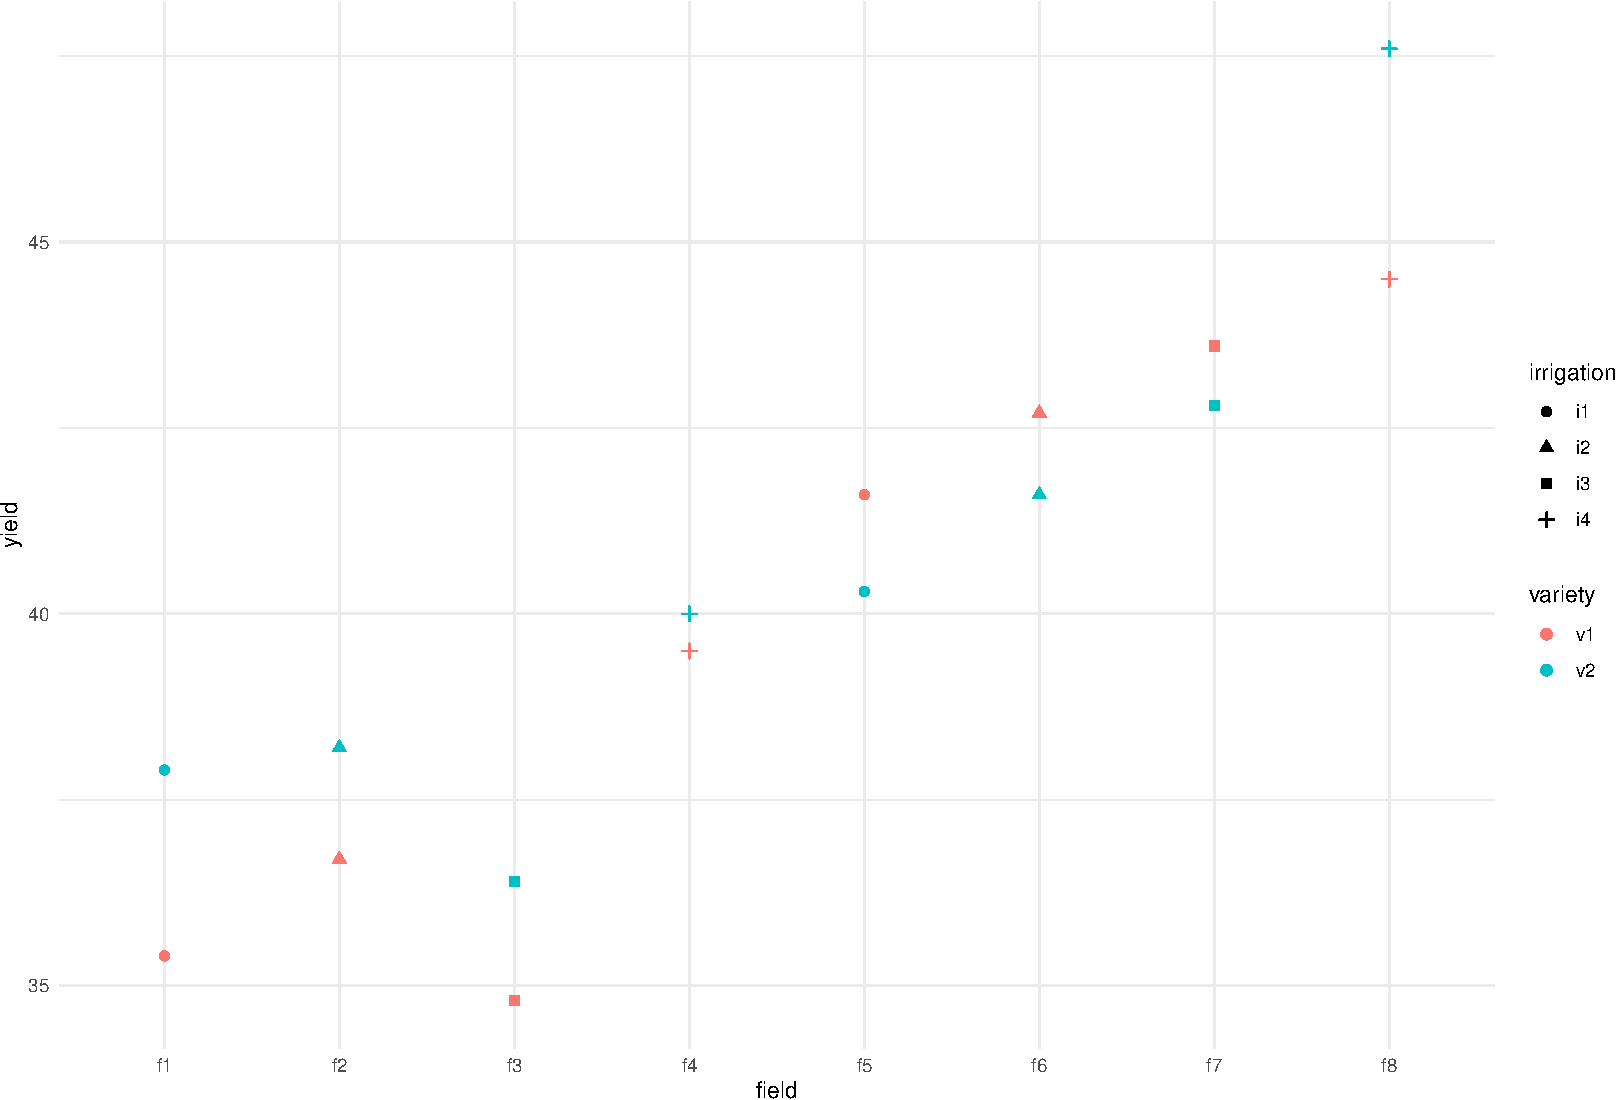
\includegraphics{week11p2_files/figure-beamer/unnamed-chunk-2-1.pdf}
\end{frame}

\begin{frame}{}
\protect\hypertarget{section-1}{}
Both irrigation and plant variety are fixed effects, but the field is
clearly a random effect (\textbf{Why so?}).

We must also consider the interaction between field and variety, which
is necessarily also a random effect because one of the two components is
random.
\end{frame}

\begin{frame}{}
\protect\hypertarget{section-2}{}
The fullest model that we might consider is: \[
  y_{ijk} = \mu + r_i + v_j + (rv)_{ij} + f_k + (vf)_{jk} + \varepsilon_{ijk},
\] where

\begin{itemize}
\item $\mu$ is a fixed model intercept,
\item $r_i$ is the fixed effect for irrigation that ranges over $i \in \{1,\ldots,4\}$ levels,
\item $v_j$ is the fixed effect for plant variety that ranges over $j \in \{1,2\}$ levels,
\item $(rv)_{ij}$ is the fixed effect interaction between irrigation and plant variety with an index ranging over $i$ and $j$,
\item $f_k$ is the random effect for field for which there are 8 realizations each indexed by $k$,
\item $(vf)_{jk}$ is the random effect interaction between plant variety and field with an index ranging over $j$ and $k$, and 
\item $\varepsilon$ is an error term for each observation.
\end{itemize}
\end{frame}

\begin{frame}[fragile]{}
\protect\hypertarget{section-3}{}
We consider normal distributions for the random effect terms that are
indexed by single variance parameters \(\sigma^2_f\), \(\sigma^2_{vf}\),
and \(\sigma^2_\varepsilon\).

Note that there is no irrigation and field interaction terms in this
model. This is because it would not be possible to estimate this effect
since only one type of irrigation method is assigned to a field.

We try to fit this model as follows:

\vspace{12pt}
\small

\begin{Shaded}
\begin{Highlighting}[]
\NormalTok{lmod }\OtherTok{\textless{}{-}} \FunctionTok{lmer}\NormalTok{(yield }\SpecialCharTok{\textasciitilde{}}\NormalTok{ irrigation }\SpecialCharTok{*}\NormalTok{ variety }\SpecialCharTok{+}\NormalTok{ (}\DecValTok{1}\SpecialCharTok{|}\NormalTok{field) }\SpecialCharTok{+} 
\NormalTok{             (}\DecValTok{1}\SpecialCharTok{|}\NormalTok{field}\SpecialCharTok{:}\NormalTok{variety), }\AttributeTok{data =}\NormalTok{ irrigation)}
\end{Highlighting}
\end{Shaded}

\begin{verbatim}
Error: number of levels of each grouping factor must 
be < number of observations (problems: field:variety)
\end{verbatim}

\vspace{12pt}
\normalsize

This failed because it is not possible to distinguish the variety within
field variation.
\end{frame}

\begin{frame}[fragile]{}
\protect\hypertarget{section-4}{}
We resort to a simpler model that omits the variety by field interaction
random effect: \[
  y_{ijk} = \mu + r_i + v_j + (rv)_{ij} + f_k + \varepsilon_{ijk}
\]

\vspace{12pt}

\begin{Shaded}
\begin{Highlighting}[]
\NormalTok{lmod }\OtherTok{\textless{}{-}} \FunctionTok{lmer}\NormalTok{(yield }\SpecialCharTok{\textasciitilde{}}\NormalTok{ irrigation }\SpecialCharTok{*}\NormalTok{ variety }\SpecialCharTok{+}\NormalTok{ (}\DecValTok{1}\SpecialCharTok{|}\NormalTok{field), }
             \AttributeTok{data =}\NormalTok{ irrigation)}
\end{Highlighting}
\end{Shaded}
\end{frame}

\begin{frame}[fragile]{}
\protect\hypertarget{section-5}{}
\small

\begin{Shaded}
\begin{Highlighting}[]
\FunctionTok{sumary}\NormalTok{(lmod)}
\end{Highlighting}
\end{Shaded}

\begin{verbatim}
## Fixed Effects:
##                        coef.est coef.se
## (Intercept)            38.50     3.03  
## irrigationi2            1.20     4.28  
## irrigationi3            0.70     4.28  
## irrigationi4            3.50     4.28  
## varietyv2               0.60     1.45  
## irrigationi2:varietyv2 -0.40     2.05  
## irrigationi3:varietyv2 -0.20     2.05  
## irrigationi4:varietyv2  1.20     2.05  
## 
## Random Effects:
##  Groups   Name        Std.Dev.
##  field    (Intercept) 4.02    
##  Residual             1.45    
## ---
## number of obs: 16, groups: field, 8
## AIC = 65.4, DIC = 91.8
## deviance = 68.6
\end{verbatim}
\end{frame}

\begin{frame}{}
\protect\hypertarget{section-6}{}
We can see that the largest variance component is that due to the field
effect, with \(\hat\sigma_f = 4.03\) compared to
\(\hat\sigma_\varepsilon = 1.45\).

The relatively large standard errors compared to the fixed effect
estimates suggest that there may be no significant fixed effects.

Wait, no p-values? See Ben Bolker's
\href{https://bbolker.github.io/mixedmodels-misc/glmmFAQ.html\#why-doesnt-lme4-display-denominator-degrees-of-freedomp-values-what-other-options-do-i-have}{GLMM
FAQ} document and Douglas Bates's
\href{https://stat.ethz.ch/pipermail/r-help/2006-May/094765.html}{commentary
on this issue}.
\end{frame}

\begin{frame}[fragile]{}
\protect\hypertarget{section-7}{}
We can check this sequentially using a backwards model selection
procedure with F-tests with adjusted degrees of freedom:

\vspace{12pt}
\tiny

\begin{Shaded}
\begin{Highlighting}[]
\FunctionTok{library}\NormalTok{(pbkrtest)}
\NormalTok{lmoda }\OtherTok{\textless{}{-}} \FunctionTok{lmer}\NormalTok{(yield }\SpecialCharTok{\textasciitilde{}}\NormalTok{ irrigation }\SpecialCharTok{+}\NormalTok{ variety }\SpecialCharTok{+}\NormalTok{ (}\DecValTok{1}\SpecialCharTok{|}\NormalTok{field), }\AttributeTok{data=}\NormalTok{irrigation)}
\FunctionTok{KRmodcomp}\NormalTok{(lmod, lmoda)}
\end{Highlighting}
\end{Shaded}

\begin{verbatim}
## large : yield ~ irrigation * variety + (1 | field)
## small : yield ~ irrigation + variety + (1 | field)
##         stat    ndf    ddf F.scaling p.value
## Ftest 0.2452 3.0000 4.0000         1  0.8612
\end{verbatim}

\vspace{12pt}
\normalsize

We find there is no significant interaction term.
\end{frame}

\begin{frame}[fragile]{}
\protect\hypertarget{section-8}{}
We can now test each of the main effects starting with the fixed effect
for plant variety:

\vspace{12pt}
\tiny

\begin{Shaded}
\begin{Highlighting}[]
\NormalTok{lmodi }\OtherTok{\textless{}{-}} \FunctionTok{lmer}\NormalTok{(yield }\SpecialCharTok{\textasciitilde{}}\NormalTok{ irrigation }\SpecialCharTok{+}\NormalTok{ (}\DecValTok{1}\SpecialCharTok{|}\NormalTok{field), irrigation)}
\FunctionTok{KRmodcomp}\NormalTok{(lmoda, lmodi)}
\end{Highlighting}
\end{Shaded}

\begin{verbatim}
## large : yield ~ irrigation + variety + (1 | field)
## small : yield ~ irrigation + (1 | field)
##         stat    ndf    ddf F.scaling p.value
## Ftest 1.5782 1.0000 7.0000         1  0.2493
\end{verbatim}

\vspace{12pt}
\normalsize

Dropping variety from the model seems reasonable since the p-value of
0.25 is large. We can test irrigation in a similar manner:

\vspace{12pt}
\tiny

\begin{Shaded}
\begin{Highlighting}[]
\NormalTok{lmodv }\OtherTok{\textless{}{-}} \FunctionTok{lmer}\NormalTok{(yield }\SpecialCharTok{\textasciitilde{}}\NormalTok{ variety }\SpecialCharTok{+}\NormalTok{ (}\DecValTok{1}\SpecialCharTok{|}\NormalTok{field), irrigation)}
\FunctionTok{KRmodcomp}\NormalTok{(lmoda, lmodv)}
\end{Highlighting}
\end{Shaded}

\begin{verbatim}
## large : yield ~ irrigation + variety + (1 | field)
## small : yield ~ variety + (1 | field)
##         stat    ndf    ddf F.scaling p.value
## Ftest 0.3882 3.0000 4.0000         1  0.7685
\end{verbatim}

\vspace{12pt}
\normalsize

Irrigation also fails to be significant.
\end{frame}

\begin{frame}[fragile]{}
\protect\hypertarget{section-9}{}
We should check the diagnostic plots to make sure there is nothing
amiss:

\vspace{12pt}
\tiny

\begin{Shaded}
\begin{Highlighting}[]
\FunctionTok{par}\NormalTok{(}\AttributeTok{mfrow =} \FunctionTok{c}\NormalTok{(}\DecValTok{1}\NormalTok{,}\DecValTok{2}\NormalTok{))}
\FunctionTok{plot}\NormalTok{(}\FunctionTok{fitted}\NormalTok{(lmod), }\FunctionTok{residuals}\NormalTok{(lmod), }\AttributeTok{xlab=}\StringTok{"Fitted"}\NormalTok{, }\AttributeTok{ylab=}\StringTok{"Residuals"}\NormalTok{, }\AttributeTok{pch =} \DecValTok{19}\NormalTok{)}
\FunctionTok{qqnorm}\NormalTok{(}\FunctionTok{residuals}\NormalTok{(lmod), }\AttributeTok{main=}\StringTok{""}\NormalTok{, }\AttributeTok{pch =} \DecValTok{19}\NormalTok{)}
\end{Highlighting}
\end{Shaded}

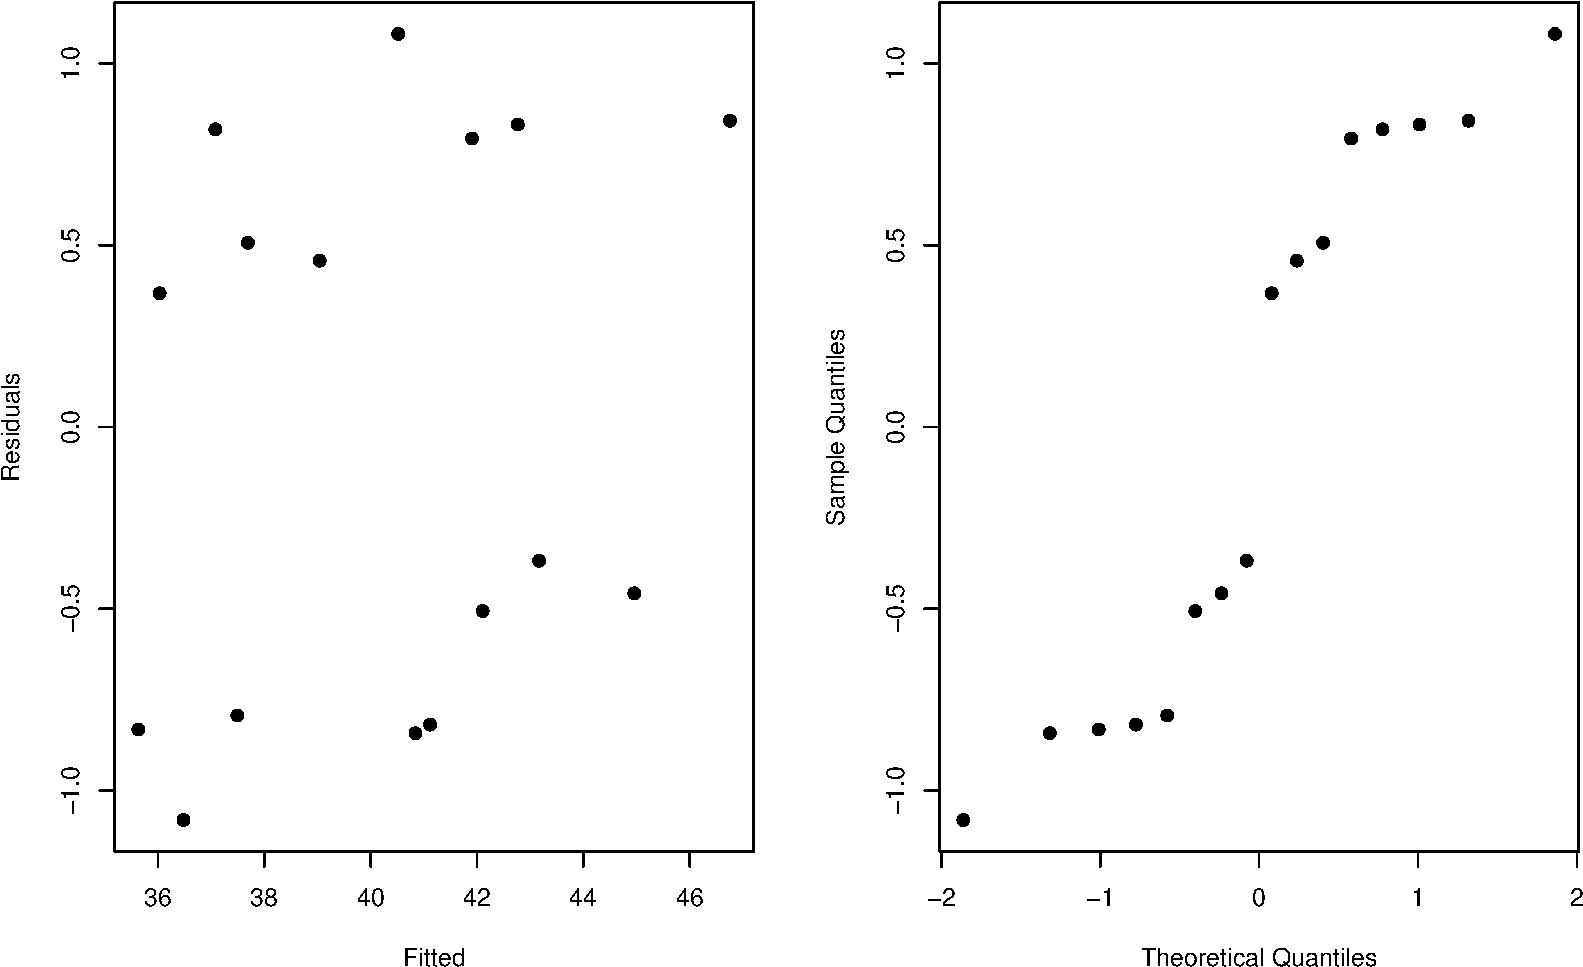
\includegraphics{week11p2_files/figure-beamer/unnamed-chunk-9-1.pdf}
\end{frame}

\begin{frame}[fragile]{}
\protect\hypertarget{section-10}{}
We can see that there is no problem with the nonconstant variance, but
that the residuals indicate a bimodal distribution caused by the pairs
of observations in each field. This type of divergence from normality is
unlikely to cause any major problems with the estimation and inference.

We can test the random effects like this:

\vspace{12pt}
\tiny

\begin{Shaded}
\begin{Highlighting}[]
\FunctionTok{library}\NormalTok{(RLRsim)}
\FunctionTok{exactRLRT}\NormalTok{(lmod)}
\end{Highlighting}
\end{Shaded}

\begin{verbatim}
## 
##  simulated finite sample distribution of RLRT.
##  
##  (p-value based on 10000 simulated values)
## 
## data:  
## RLRT = 6.1118, p-value = 0.0095
\end{verbatim}

\vspace{12pt}
\normalsize

We see that the fields do seem to vary as the result is clearly
significant.
\end{frame}

\begin{frame}{Example of nested random effects}
\protect\hypertarget{example-of-nested-random-effects}{}
Consistency between laboratory tests is important and yet the results
may depend on who did the test and where the test was performed.

In an experiment to test levels of consistency, a large jar of dried egg
powder was divided up into a number of samples.

Because the powder was homogenized, the fat content of the samples is
the same, but this fact is withheld from the laboratories.
\end{frame}

\begin{frame}[fragile]{Follow the randomness}
\protect\hypertarget{follow-the-randomness}{}
Four samples were sent to each of six laboratories.

Two of the samples were labeled as G and two as H, although in fact they
were identical.

The laboratories were instructed to give two samples to two different
technicians.

The technicians were then instructed to divide their samples into two
parts and measure the fat content of each.

So each laboratory reported eight measures, each technician four
measures, that is, two replicated measures on each of two samples. The
data comes from Bliss (1967):

\vspace{12pt}
\tiny

\begin{Shaded}
\begin{Highlighting}[]
\FunctionTok{data}\NormalTok{(eggs)}
\FunctionTok{head}\NormalTok{(eggs, }\DecValTok{3}\NormalTok{)}
\end{Highlighting}
\end{Shaded}

\begin{verbatim}
##    Fat Lab Technician Sample
## 1 0.62   I        one      G
## 2 0.55   I        one      G
## 3 0.34   I        one      H
\end{verbatim}
\end{frame}

\begin{frame}[fragile]{}
\protect\hypertarget{section-11}{}
\tiny

\begin{Shaded}
\begin{Highlighting}[]
\FunctionTok{ggplot}\NormalTok{(eggs, }\FunctionTok{aes}\NormalTok{(}\AttributeTok{y=}\NormalTok{Fat, }\AttributeTok{x=}\NormalTok{Lab, }\AttributeTok{color=}\NormalTok{Technician, }\AttributeTok{shape=}\NormalTok{Sample)) }\SpecialCharTok{+} 
  \FunctionTok{geom\_point}\NormalTok{(}\AttributeTok{size =} \DecValTok{2}\NormalTok{, }\AttributeTok{position =} \FunctionTok{position\_jitter}\NormalTok{(}\AttributeTok{width=}\FloatTok{0.1}\NormalTok{, }\AttributeTok{height=}\FloatTok{0.0}\NormalTok{)) }\SpecialCharTok{+} 
  \FunctionTok{scale\_color\_grey}\NormalTok{() }\SpecialCharTok{+} 
  \FunctionTok{theme\_minimal}\NormalTok{()}
\end{Highlighting}
\end{Shaded}

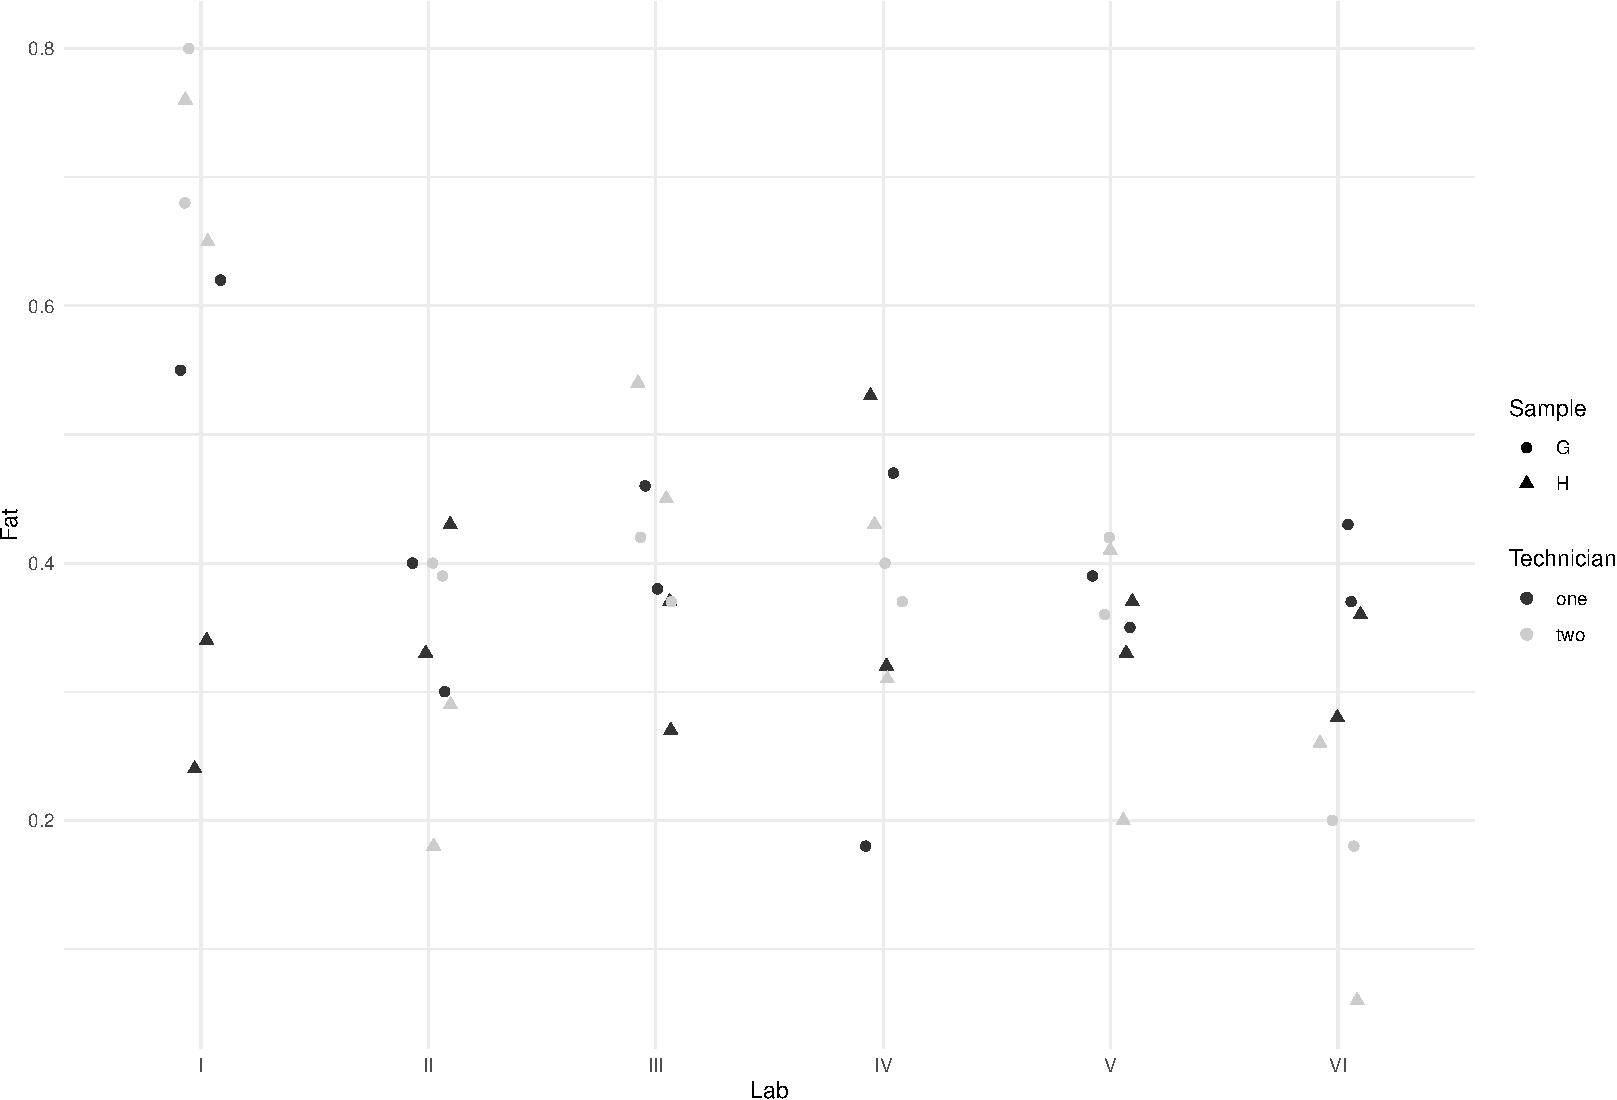
\includegraphics{week11p2_files/figure-beamer/unnamed-chunk-11-1.pdf}
\end{frame}

\begin{frame}{}
\protect\hypertarget{section-12}{}
Our model is \[
  y_{ijkl} = \mu + L_i + T_{ij} + S_{ijk} + \varepsilon_{ijkl}
\] where,

\begin{itemize}
\item $\mu$ is a fixed model intercept,
\item $L_i$ is the random effect for lab for which there are 6 realizations each indexed by $i$,
\item $T_{ij}$ is the random effect for technician nested within lab for which there are 2 realizations each indexed by $j$ within each lab $i$, 
\item $S_{ijk}$ is the random effect for sample nested within technician nested within lab. There are four realizations each indexed by $k$ by each technician $j$ within each lab $i$, and
\item $\varepsilon$ is an error term for each observation.
\end{itemize}
\end{frame}

\begin{frame}[fragile]{}
\protect\hypertarget{section-13}{}
This can be fit with:

\vspace{12pt}
\tiny

\begin{Shaded}
\begin{Highlighting}[]
\NormalTok{cmod }\OtherTok{\textless{}{-}} \FunctionTok{lmer}\NormalTok{(Fat }\SpecialCharTok{\textasciitilde{}} \DecValTok{1} \SpecialCharTok{+}\NormalTok{ (}\DecValTok{1}\SpecialCharTok{|}\NormalTok{Lab) }\SpecialCharTok{+}\NormalTok{ (}\DecValTok{1}\SpecialCharTok{|}\NormalTok{Lab}\SpecialCharTok{:}\NormalTok{Technician) }\SpecialCharTok{+}\NormalTok{  (}\DecValTok{1}\SpecialCharTok{|}\NormalTok{Lab}\SpecialCharTok{:}\NormalTok{Technician}\SpecialCharTok{:}\NormalTok{Sample), }
             \AttributeTok{data=}\NormalTok{eggs) }
\FunctionTok{sumary}\NormalTok{(cmod)}
\end{Highlighting}
\end{Shaded}

\begin{verbatim}
## Fixed Effects:
## coef.est  coef.se 
##     0.39     0.04 
## 
## Random Effects:
##  Groups                Name        Std.Dev.
##  Lab:Technician:Sample (Intercept) 0.06    
##  Lab:Technician        (Intercept) 0.08    
##  Lab                   (Intercept) 0.08    
##  Residual                          0.08    
## ---
## number of obs: 48, groups: Lab:Technician:Sample, 24; Lab:Technician, 12; Lab, 6
## AIC = -54.2, DIC = -73.3
## deviance = -68.8
\end{verbatim}
\end{frame}

\begin{frame}{}
\protect\hypertarget{section-14}{}
So we have that the estimated variance components are all similar in
magnitude.

The lack of consistency in measures of fat content can be ascribed to
variance between labs, technicians, measurement due to different
labeling, and measurement error.

Although the data has a natural hierarchical structure which suggests a
particular order of testing, we might reasonably wonder which of the
components contribute substantially to the overall variation.
\end{frame}

\begin{frame}[fragile]{}
\protect\hypertarget{section-15}{}
A look at the confidence intervals reveals the problem:

\vspace{12pt}
\tiny

\begin{Shaded}
\begin{Highlighting}[]
\FunctionTok{confint}\NormalTok{(cmod, }\AttributeTok{method=}\StringTok{"boot"}\NormalTok{)}
\end{Highlighting}
\end{Shaded}

\begin{verbatim}
##                  2.5 %     97.5 %
## .sig01      0.00000000 0.09628667
## .sig02      0.00000000 0.13598404
## .sig03      0.00000000 0.14699799
## .sigma      0.05966933 0.10614784
## (Intercept) 0.31175286 0.47064824
\end{verbatim}

\vspace{12pt}
\normalsize

We might drop any of the three random effect terms but it is not
possible to be sure which is best to go.

It is safest to conclude there is some variation in the fat measurement
coming from all three sources.
\end{frame}

\begin{frame}{Repeated measures and longitudinal data}
\protect\hypertarget{repeated-measures-and-longitudinal-data}{}
In repeated measures designs there are several individuals (or units)
under study and multiple measurements are taken repeatedly on each
individual.

When these repeated measurements are taken over time, it is called a
longitudinal study or, in some applications, a panel study.

Typically there are various covariates concerning the individual that
are also recorded and interest centers on how the response depends on
these covariates over time. Often it is reasonable to believe that the
response of each individual has several components:

\begin{itemize}
\item
  a fixed effect, which is a function of the covariates;
\item
  a random effect, which expresses the variation between individuals;
\item
  and an error, which is due to measurement or unrecorded variables.
\end{itemize}
\end{frame}

\begin{frame}{}
\protect\hypertarget{section-16}{}
In a repeated measures design we will suppose that each individual has a
response \(y_i\) which is now a vector of length \(n_i\) and is modeled
conditionally on the random effect \(b_i\) as \[
  y_i | b_i \sim N(X_i\beta + Z_i b_i, \sigma^2 \Lambda_i).
\] Note that this is a very similar model used in the linear
mixed-effects model construction above, with the exception that we now
allow for the individuals to have a more general covariance structure
\(\Lambda_i\).

As before, we will assume that \(b_i \sim N(0, \sigma^2 D)\) so that \[
  y_i \sim N(X_i\beta, \Sigma_i)
\] where \(\Sigma_i = \sigma^2(\Lambda_i + Z_iDZ_i^T)\).
\end{frame}

\begin{frame}{}
\protect\hypertarget{section-17}{}
Now suppose that we have \(N\) individuals and assume that the
measurement errors and random effects between individuals are
uncorrelated. Then we can combine the data as: \[
  Y = \left[\begin{array}{c}
  y_1 \\
  y_2 \\
  \vdots \\
  y_N
  \end{array}\right], \qquad 
  X = \left[\begin{array}{c}
  X_1 \\
  X_2 \\
  \vdots \\
  X_N
  \end{array}\right], \qquad
  B = \left[\begin{array}{c}
  b_1 \\
  b_2 \\
  \vdots \\
  b_N
  \end{array}\right],
\] and

\begin{itemize}
\item
  \(\tilde{D} = \text{diag}(D,D,\ldots,D)\),
\item
  \(Z = \text{diag}(Z_1,Z_2,\ldots,Z_N)\),
\item
  \(\Sigma = \text{diag}(\Sigma_1,\Sigma_2,\ldots,\Sigma_N)\), and
\item
  \(\Lambda = \text{diag}(\Lambda_1,\Lambda_2,\ldots,\Lambda_N)\), where
\end{itemize}

\(y_i \in \mathbb{R}^{n_i}\), \(X_i \in \mathbb{R}^{n_i\times p}\),
\(\beta \in \mathbb{R}^p\), \(b_i \in \mathbb{R}^{q}\),
\(Z_i \in \mathbb{R}^{n_i \times q}\), and the rest of the quantities in
the above follow from these specifications.
\end{frame}

\begin{frame}{}
\protect\hypertarget{section-18}{}
With this setup we can write the model as \[
  Y \sim N(X\beta, \Sigma) \qquad \text{where} \qquad \Sigma = \sigma^2(\Lambda + Z\tilde{D}Z^T).
\]

The log-likelihood for the data is then computed as previously and
estimation, testing, standard errors and confidence intervals all follow
using standard likelihood theory as before.

There is no strong distinction between repeated measures methodology and
the methodology of linear mixed-effects models.
\end{frame}

\begin{frame}[fragile]{Example: Panel Study of Income Dynamics}
\protect\hypertarget{example-panel-study-of-income-dynamics}{}
The Panel Study of Income Dynamics (PSID), begun in 1968, is a
longitudinal study of a representative sample of U.S. individuals
described in
\href{https://onesearch.library.rice.edu/discovery/fulldisplay?vid=01RICE_INST:RICE\&search_scope=MyInst_and_CI\&tab=Everything\&docid=alma991025907119705251\&lang=en\&context=L\&adaptor=Local\%20Search\%20Engine\&query=sub,exact,Famines,AND\&mode=advanced\&offset=0}{Hill
(1992)}.

There are currently 8700 households in the study and many variables are
measured. We chose to analyze a random subset of this data, consisting
of 85 heads of household who were aged 25--39 in 1968 and had complete
data for at least 11 of the years between 1968 and 1990.

The variables included were annual income, gender, years of education
and age in 1968:

\vspace{12pt}
\tiny

\begin{Shaded}
\begin{Highlighting}[]
\FunctionTok{library}\NormalTok{(tidyverse)}
\FunctionTok{head}\NormalTok{(psid)}
\end{Highlighting}
\end{Shaded}

\begin{verbatim}
##   age educ sex income year person
## 1  31   12   M   6000   68      1
## 2  31   12   M   5300   69      1
## 3  31   12   M   5200   70      1
## 4  31   12   M   6900   71      1
## 5  31   12   M   7500   72      1
## 6  31   12   M   8000   73      1
\end{verbatim}
\end{frame}

\begin{frame}[fragile]{}
\protect\hypertarget{section-19}{}
\tiny

\begin{Shaded}
\begin{Highlighting}[]
\DocumentationTok{\#\# first 20 observations}
\NormalTok{psid20 }\OtherTok{\textless{}{-}} \FunctionTok{filter}\NormalTok{(psid, person }\SpecialCharTok{\textless{}=} \DecValTok{20}\NormalTok{)}
\FunctionTok{ggplot}\NormalTok{(psid20, }\FunctionTok{aes}\NormalTok{(}\AttributeTok{x=}\NormalTok{year, }\AttributeTok{y=}\NormalTok{income)) }\SpecialCharTok{+} 
  \FunctionTok{geom\_line}\NormalTok{() }\SpecialCharTok{+} \FunctionTok{facet\_wrap}\NormalTok{(}\SpecialCharTok{\textasciitilde{}}\NormalTok{ person) }\SpecialCharTok{+} \FunctionTok{theme\_minimal}\NormalTok{()}
\end{Highlighting}
\end{Shaded}

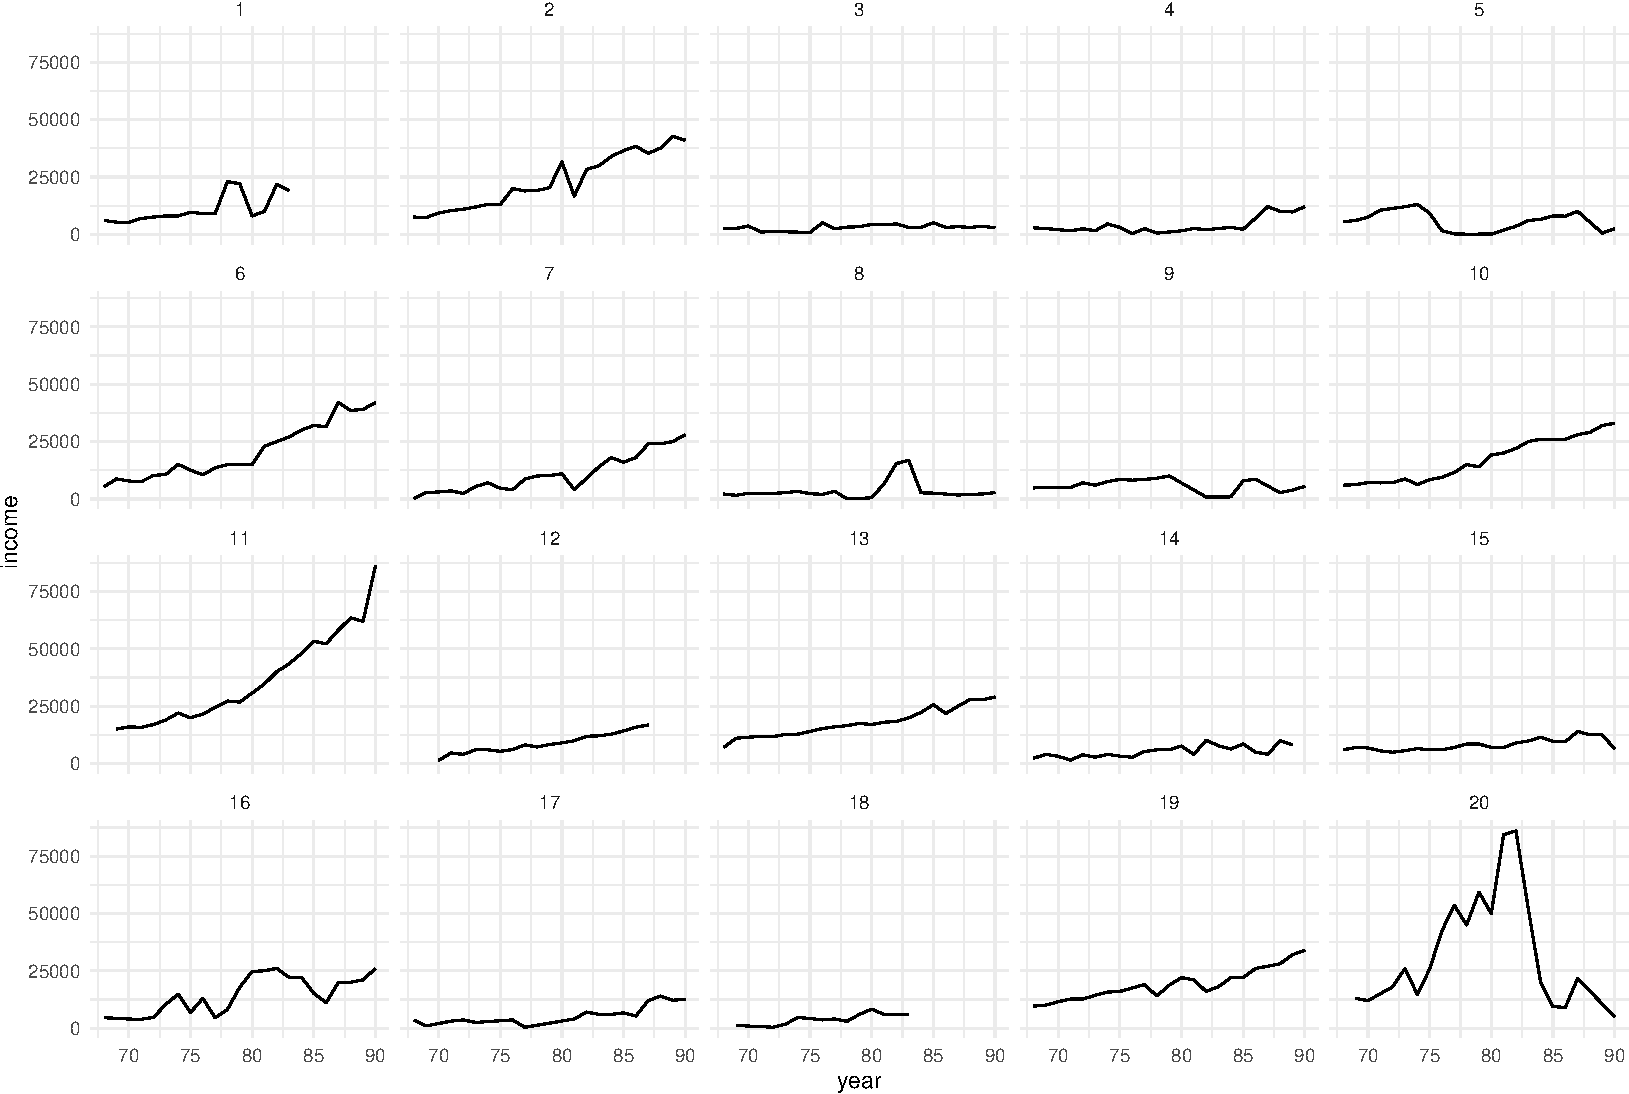
\includegraphics{week11p2_files/figure-beamer/unnamed-chunk-14-1.pdf}
\end{frame}

\begin{frame}[fragile]{}
\protect\hypertarget{section-20}{}
We see that some individuals have a slowly increasing income, typical of
someone in steady employment in the same job. Other individuals have
more erratic incomes. We can also show how the incomes vary by sex.

Income is more naturally considered on a log-scale:

\vspace{12pt}
\tiny

\begin{Shaded}
\begin{Highlighting}[]
\FunctionTok{ggplot}\NormalTok{(psid20, }\FunctionTok{aes}\NormalTok{(}\AttributeTok{x=}\NormalTok{year, }\AttributeTok{y=}\NormalTok{income}\SpecialCharTok{+}\DecValTok{100}\NormalTok{, }\AttributeTok{group=}\NormalTok{person)) }\SpecialCharTok{+} 
  \FunctionTok{geom\_line}\NormalTok{() }\SpecialCharTok{+} \FunctionTok{facet\_wrap}\NormalTok{(}\SpecialCharTok{\textasciitilde{}}\NormalTok{ sex) }\SpecialCharTok{+} \FunctionTok{scale\_y\_log10}\NormalTok{() }\SpecialCharTok{+} \FunctionTok{theme\_minimal}\NormalTok{()}
\end{Highlighting}
\end{Shaded}

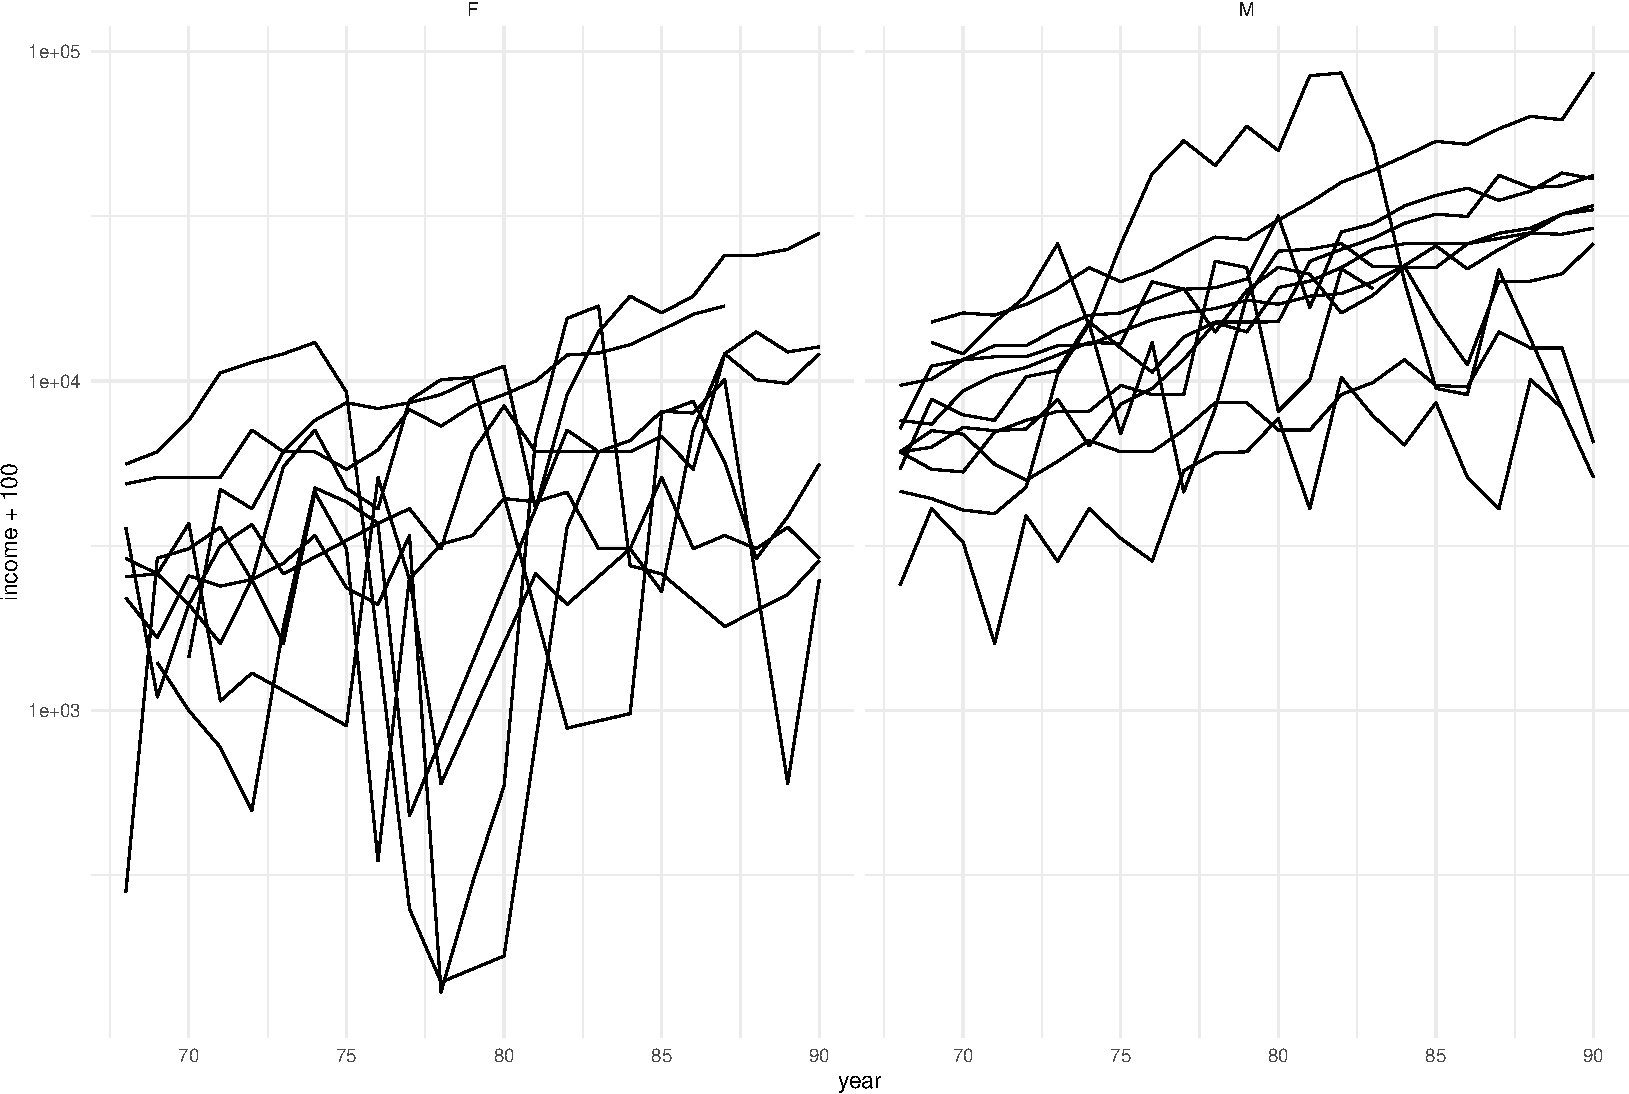
\includegraphics[width=3.5in,height=2in]{week11p2_files/figure-beamer/unnamed-chunk-15-1}
\end{frame}

\begin{frame}[fragile]{}
\protect\hypertarget{section-21}{}
We added \$100 to the income of each subject to remove the effect of
some subjects having very low incomes for short periods of time. These
cases distorted the plots without the adjustment.

We see that men's incomes are generally higher and less variable while
women's incomes are more variable, but are perhaps increasing more
quickly.

We could fit a line to each subject starting with the first:

\vspace{12pt}
\small

\begin{Shaded}
\begin{Highlighting}[]
\NormalTok{lmod }\OtherTok{\textless{}{-}} \FunctionTok{lm}\NormalTok{(}\FunctionTok{log}\NormalTok{(income) }\SpecialCharTok{\textasciitilde{}} \FunctionTok{I}\NormalTok{(year}\DecValTok{{-}78}\NormalTok{), }\AttributeTok{subset=}\NormalTok{(person}\SpecialCharTok{==}\DecValTok{1}\NormalTok{), psid)}
\FunctionTok{coef}\NormalTok{(lmod)}
\end{Highlighting}
\end{Shaded}

\begin{verbatim}
##  (Intercept) I(year - 78) 
##    9.3999568    0.0842667
\end{verbatim}
\end{frame}

\begin{frame}[fragile]{}
\protect\hypertarget{section-22}{}
Note that we have centered the predictor year at its median value so
that the intercept will represent the predicted log income in 1978 and
not the year 1900 which is nonsense (any sensible location
transformation would be appropriate, but centering with respect to the
median is perhaps most appropriate).

We now fit a line for all the subjects and plot the results:

\vspace{12pt}
\small

\begin{Shaded}
\begin{Highlighting}[]
\NormalTok{ml }\OtherTok{\textless{}{-}} \FunctionTok{lmList}\NormalTok{(}\FunctionTok{log}\NormalTok{(income) }\SpecialCharTok{\textasciitilde{}} \FunctionTok{I}\NormalTok{(year}\DecValTok{{-}78}\NormalTok{) }\SpecialCharTok{|}\NormalTok{ person, psid)}
\NormalTok{intercepts }\OtherTok{\textless{}{-}} \FunctionTok{sapply}\NormalTok{(ml,coef)[}\DecValTok{1}\NormalTok{,]}
\NormalTok{slopes }\OtherTok{\textless{}{-}} \FunctionTok{sapply}\NormalTok{(ml,coef)[}\DecValTok{2}\NormalTok{,]}
\end{Highlighting}
\end{Shaded}

\vspace{12pt}
\normalsize

The \texttt{lmList} command fits a linear model to each group within the
data, here specified by person.
\end{frame}

\begin{frame}[fragile]{}
\protect\hypertarget{section-23}{}
We can test the difference in income growth rates for men and women:

\vspace{12pt}
\small

\begin{Shaded}
\begin{Highlighting}[]
\NormalTok{psex }\OtherTok{\textless{}{-}}\NormalTok{ psid}\SpecialCharTok{$}\NormalTok{sex[}\FunctionTok{match}\NormalTok{(}\DecValTok{1}\SpecialCharTok{:}\DecValTok{85}\NormalTok{,psid}\SpecialCharTok{$}\NormalTok{person)]}
\FunctionTok{t.test}\NormalTok{(slopes[psex}\SpecialCharTok{==}\StringTok{"M"}\NormalTok{],slopes[psex}\SpecialCharTok{==}\StringTok{"F"}\NormalTok{])}
\end{Highlighting}
\end{Shaded}

\begin{verbatim}
## 
##  Welch Two Sample t-test
## 
## data:  slopes[psex == "M"] and slopes[psex == "F"]
## t = -2.3786, df = 56.736, p-value = 0.02077
## alternative hypothesis: true difference in means is not equal to 0
## 95 percent confidence interval:
##  -0.05916871 -0.00507729
## sample estimates:
##  mean of x  mean of y 
## 0.05691046 0.08903346
\end{verbatim}

\vspace{12pt}
\normalsize

We see that women have a significantly higher growth rate than men.
\end{frame}

\begin{frame}[fragile]{}
\protect\hypertarget{section-24}{}
We can also compare the incomes at the intercept (which is 1978):

\vspace{12pt}
\small

\begin{Shaded}
\begin{Highlighting}[]
\FunctionTok{t.test}\NormalTok{(intercepts[psex}\SpecialCharTok{==}\StringTok{"M"}\NormalTok{],intercepts[psex}\SpecialCharTok{==}\StringTok{"F"}\NormalTok{])}
\end{Highlighting}
\end{Shaded}

\begin{verbatim}
## 
##  Welch Two Sample t-test
## 
## data:  intercepts[psex == "M"] and intercepts[psex == "F"]
## t = 8.2199, df = 79.719, p-value = 3.065e-12
## alternative hypothesis: true difference in means is not equal to 0
## 95 percent confidence interval:
##  0.8738792 1.4322218
## sample estimates:
## mean of x mean of y 
##  9.382325  8.229275
\end{verbatim}

\vspace{12pt}
\normalsize

We see that men have significantly higher incomes.
\end{frame}

\begin{frame}{Response feature analysis}
\protect\hypertarget{response-feature-analysis}{}
This is an example of a response feature analysis.

It requires choosing an important characteristic. We have chosen two
here: the slope and the intercept. For many datasets, this is not an
easy choice and at least some information is lost by doing this.

Response feature analysis is attractive because of its simplicity. By
extracting a univariate response for each individual, we are able to use
a wide array of well-known statistical techniques.

However, it is not the most efficient use of the data as all the
additional information besides the chosen response feature is discarded.
Notice that having additional data on each subject would be of limited
value.
\end{frame}

\begin{frame}{}
\protect\hypertarget{section-25}{}
Suppose that the income change over time can be partly predicted by the
subject's age, sex and educational level.

We do not expect a perfect fit. Clearly there are other factors that
will affect a subject's income. These factors may cause the income to be
generally higher or lower or they may cause the income to grow at a
faster or slower rate.

We can model this variation with a random intercept and slope,
respectively, for each subject.

We also expect that there will be some year-to-year variation within
each subject. For simplicity, let us initially assume that this error is
homogeneous and uncorrelated, that is, \(\Lambda_i = I\).
\end{frame}

\begin{frame}[fragile]{}
\protect\hypertarget{section-26}{}
We also center the year to aid interpretation as before. We may express
these notions in the model:

\vspace{12pt}
\tiny

\begin{Shaded}
\begin{Highlighting}[]
\NormalTok{psid}\SpecialCharTok{$}\NormalTok{cyear }\OtherTok{\textless{}{-}}\NormalTok{ psid}\SpecialCharTok{$}\NormalTok{year }\SpecialCharTok{{-}} \DecValTok{78}
\NormalTok{mmod }\OtherTok{\textless{}{-}} \FunctionTok{lmer}\NormalTok{(}\FunctionTok{log}\NormalTok{(income) }\SpecialCharTok{\textasciitilde{}}\NormalTok{ cyear}\SpecialCharTok{*}\NormalTok{sex }\SpecialCharTok{+}\NormalTok{ age }\SpecialCharTok{+}\NormalTok{ educ }\SpecialCharTok{+}\NormalTok{ (cyear}\SpecialCharTok{|}\NormalTok{person), psid)}
\end{Highlighting}
\end{Shaded}

\vspace{12pt}
\normalsize

This model can be written as \begin{align*}
  &\log(\text{income})_{ij} = 
    \mu + \beta_y\text{year}_j + \beta_g \text{sex}_i + \beta_{yg}\text{sex}_i*\text{year}_j + \beta_e\text{education}_i \\
    &\qquad+ \beta_a\text{age}_i + \gamma_i^0 + \gamma_i^1 \text{year}_j + \varepsilon_{ij}
\end{align*} where \(i\) indexes the individuals and \(j\) indexes the
years, and \(\log\) is the natural logarithm. We have: \[
\begin{pmatrix}
  \gamma_j^0 \\
  \gamma_j^1
\end{pmatrix} \sim N(0, \sigma^2D)
\]
\end{frame}

\begin{frame}[fragile]{}
\protect\hypertarget{section-27}{}
\small

\begin{Shaded}
\begin{Highlighting}[]
\FunctionTok{sumary}\NormalTok{(mmod, }\AttributeTok{digits=}\DecValTok{3}\NormalTok{)}
\end{Highlighting}
\end{Shaded}

\begin{verbatim}
## Fixed Effects:
##             coef.est coef.se
## (Intercept)  6.674    0.543 
## cyear        0.085    0.009 
## sexM         1.150    0.121 
## age          0.011    0.014 
## educ         0.104    0.021 
## cyear:sexM  -0.026    0.012 
## 
## Random Effects:
##  Groups   Name        Std.Dev. Corr  
##  person   (Intercept) 0.531          
##           cyear       0.049    0.187 
##  Residual             0.684          
## ---
## number of obs: 1661, groups: person, 85
## AIC = 3839.8, DIC = 3751.2
## deviance = 3785.5
\end{verbatim}
\end{frame}

\begin{frame}{}
\protect\hypertarget{section-28}{}
We now analyze this summary table. Lets start with the fixed effects. We
see that:

\begin{itemize}
\tightlist
\item
  income increases about 10\% for each additional year of education. We
  see that age does not appear to be significant.
\item
  For males, the reference level in this example, income increases about
  7.2\% a year, while for women, it increases about 7.2\% + 1.3\% =
  8.5\% a year.
\item
  We see that, for this data, the incomes of women are exp(-0.575) =
  0.563 times higher (far lower!).
\end{itemize}
\end{frame}

\begin{frame}{}
\protect\hypertarget{section-29}{}
Now the random effects. We see that:

\begin{itemize}
\tightlist
\item
  We know the mean for males and females, but individuals will vary
  about this. The standard deviation for the intercept and slope are
  0.531 and 0.049 (\(\sigma\sqrt{D_{11}}\) and \(\sigma\sqrt{D_{22}}\)),
  respectively. These have a correlation of 0.187
  (cor\((\gamma^0,\gamma^1)\)).
\item
  There is some additional variation in the measurement not so far
  accounted for having standard deviation of 0.684
  (sd(\(\varepsilon_{ij}\))).
\item
  We see that the variation in increase in income is relatively small
  while the variation in overall income between individuals is quite
  large.
\item
  Furthermore, given the large residual variation, there is a large
  year-to-year variation in incomes.
\end{itemize}
\end{frame}

\end{document}
